\documentclass[aspectratio=169, 10pt]{beamer}

% ---------- Tema y colores ----------
\usetheme{default}
\usecolortheme{default}
\setbeamertemplate{navigation symbols}{}
\setbeamertemplate{footline}[frame number]
\setbeamertemplate{frametitle continuation}{}

\definecolor{StanfordRed}{RGB}{140,21,21}
\definecolor{StanfordGray}{RGB}{77,77,77}
\definecolor{LightGray}{RGB}{240,240,240}
\definecolor{AccentBlue}{RGB}{0,84,166}
\definecolor{AccentGreen}{RGB}{0,130,100}
\definecolor{UCMBlue}{RGB}{4, 171, 226}
\definecolor{UCMNavy}{RGB}{20, 65, 134}

\setbeamercolor{frametitle}{fg=white, bg=UCMBlue}
\setbeamercolor{title}{fg=white}
\setbeamercolor{author}{fg=white}
\setbeamercolor{institute}{fg=white!80}
\setbeamercolor{structure}{fg=UCMBlue}
\setbeamercolor{block title}{bg=UCMBlue!15!white, fg=UCMBlue}
\setbeamercolor{block body}{bg=LightGray}
\setbeamercolor{alerted text}{fg=UCMBlue}
\setbeamercolor{example text}{fg=UCMBlue}

\setbeamerfont{frametitle}{series=\bfseries, size=\large}
\setbeamerfont{title}{series=\bfseries, size=\LARGE}
\setbeamerfont{block title}{series=\bfseries}

% ---------- Paquetes ----------
\usepackage[utf8]{inputenc}
\usepackage[T1]{fontenc}
\usepackage[provide=*,spanish]{babel}
\usepackage{amsmath, amssymb, bm}
\usepackage{algorithmic}
\usepackage{tikz}
\usepackage{pgfplots}
\pgfplotsset{compat=1.18}
\usetikzlibrary{arrows.meta, shapes.geometric, positioning, fit, calc,
	decorations.pathreplacing, backgrounds, shadows, patterns}
\usepackage{booktabs}
\usepackage{xcolor}
\usepackage{multicol}
\usepackage{tcolorbox}
\tcbuselibrary{skins, breakable}

% ---------- Comandos útiles ----------
\newcommand{\R}{\mathbb{R}}
\newcommand{\E}{\mathbb{E}}
\newcommand{\Var}{\operatorname{Var}}
\newcommand{\MSE}{\operatorname{MSE}}
\newcommand{\Bias}{\operatorname{Sesgo}}
\newcommand{\y}{\bm{y}}
\newcommand{\X}{\bm{X}}
\newcommand{\bbeta}{\bm{\beta}}

\newcommand{\formula}[1]{%
	\begin{tcolorbox}[colback=UCMBlue!8, colframe=UCMBlue, arc=4pt,
		boxsep=2pt, left=6pt, right=6pt, top=3pt, bottom=3pt]
		#1
	\end{tcolorbox}
}

% ---------- Portada ----------
\title{\textbf{Machine Learning}}
\subtitle{MDS-211 Magister en Data Science}
\author{Sergio Hernández\\ shernandez@ucm.cl}
\institute{ \begin{tikzpicture}
		\clip [rounded corners=1cm] (0,0) rectangle (4,2);
		\node[anchor=south west, inner sep=0pt] at (0,0) 
		{\includegraphics[width=4cm, height=2cm]{figures/mindslab.png}};
	\end{tikzpicture}
	\\ \textbf{Universidad Católica del Maule}}
\date{}


\begin{document}
% --- Título ---
{
	\setbeamertemplate{background}{
		\begin{tikzpicture}[remember picture, overlay]
			\fill[UCMBlue] (current page.south west) rectangle (current page.north east);
			\fill[UCMBlue!70!black, opacity=0.5]
			(current page.south west) -- ++(0,3) -- ++(18,0) -- cycle;
			\foreach \i in {1,...,40}{
				\fill[white, opacity=0.04]
				({random()*17}, {random()*10}) circle ({random()*0.3});
			}
		\end{tikzpicture}
	}
	\begin{frame}[plain]
		\vspace{1.2cm}
		\titlepage
		\begin{tikzpicture}[remember picture, overlay]
			\node[white, opacity=0.15, font=\fontsize{80}{80}\selectfont] 
			at (current page.east) [xshift=-2cm] {$\Sigma$};
		\end{tikzpicture}
	\end{frame}
}


%=====================================================================
\section{Motivaci\'on: Sesgo y Varianza}
%=====================================================================

\begin{frame}
\frametitle{Descomposici\'on Sesgo--Varianza}
El error de predicci\'on esperado de un modelo $\hat{f}(x)$ se descompone en tres t\'erminos\footnote{Hastie, T., Tibshirani, R., \& Friedman, J. (2009). \emph{The Elements of Statistical Learning}. Springer.}:
\begin{align*}
\underbrace{\text{EPE}\big(\hat{f}(x)\big)}_{\text{error esperado}} =
\underbrace{\text{Sesgo}^2\big[\hat{f}(x)\big] + \text{Var}\big[\hat{f}(x)\big]}_{\text{error reducible}}
+ \underbrace{\sigma^2}_{\text{error irreducible}}
\end{align*}
\begin{itemize}
	\item \textbf{Sesgo} (\emph{bias}): diferencia entre la predicci\'on esperada y el valor real. Surge de suposiciones demasiado simples $\Rightarrow$ \emph{sub-ajuste}.
	\pause
	\item \textbf{Varianza}: cu\'anto cambia el modelo al entrenarlo sobre un conjunto de datos distinto. Modelos muy flexibles $\Rightarrow$ \emph{sobre-ajuste}.
	\pause
	\item \textbf{Ruido} ($\sigma^2$): error inherente a los datos; no puede reducirse con ning\'un modelo.
\end{itemize}
\end{frame}

\begin{frame}
\frametitle{El compromiso Sesgo--Varianza}
\begin{center}
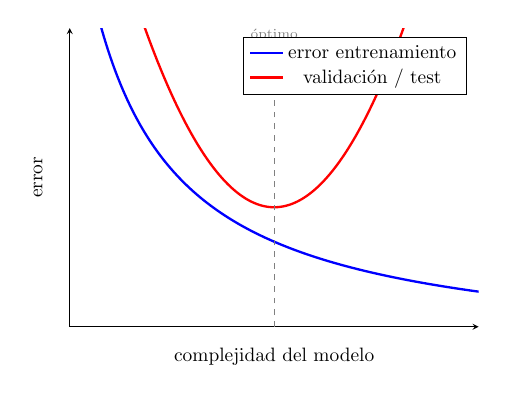
\begin{tikzpicture}[scale=.7]
    \begin{axis}[
        legend pos=north east,
        axis x line=middle,
        axis y line=middle,
        width=9cm,
        height=7cm,
        xmin= 0,
        xmax= 2,
        ymin= 0,
        ymax= 2,
        xlabel=complejidad del modelo,
        ylabel=error,
        ticks=none,
        xticklabels={,,},
        yticklabels={,,},
        x label style={at={(axis description cs:0.5,-0.05)},
                       anchor=north},
        y label style={at={(axis description cs:-0.05,0.5)},
                       anchor=south,
                       rotate=90},]
      % error de entrenamiento (decrece con la complejidad)
      \addplot[domain=0:2,samples=500,very thick,blue] {1/(x+0.3)-0.2};
      % error de validacion / test (forma de U)
      \addplot[domain=0:2, red, very thick,samples=500] {3*(x-2)*x+3.8};
      % complejidad optima
      \draw[dashed,gray] (axis cs:1,0) -- (axis cs:1,1.8);
      \node[gray] at (axis cs:1,1.95) {\scriptsize \'optimo};
      \addlegendentry{error entrenamiento}
      \addlegendentry{validaci\'on / test}
    \end{axis}
\end{tikzpicture}
\end{center}
\begin{itemize}
	\item A la izquierda domina el \textbf{sesgo} (sub-ajuste); a la derecha domina la \textbf{varianza} (sobre-ajuste).
	\item Los ensambles buscan \emph{romper} este compromiso: reducir la varianza (\emph{bagging}) o el sesgo (\emph{boosting}) sin pagar el costo del otro t\'ermino.
\end{itemize}
\end{frame}


\begin{frame}
\frametitle{La idea de los ensambles}
\begin{block}{Definici\'on}
Un \emph{ensamble} combina las predicciones de muchos modelos diversos en un \'unico predictor, generalmente m\'as exacto y robusto que cualquiera de sus miembros.
\end{block}
\pause
\begin{columns}[T]
\begin{column}{6cm}
\begin{itemize}
	\item En lugar de ajustar un \'unico modelo, se entrena una \emph{colecci\'on} de modelos y se agregan sus predicciones (promedio o votaci\'on).
	%\pause
	\item \textbf{Sabidur\'ia de las multitudes}: si cada modelo acierta mejor que el azar y sus errores son \emph{independientes}, el voto mayoritario reduce el error a medida que crece el ensamble.
\end{itemize}
\end{column}
\begin{column}{4.5cm}
\tikzstyle{block} = [draw,fill=blue!20,minimum size=2em]
\begin{center}
\begin{tikzpicture}[scale=0.8,transform shape]
\foreach \y in {1,2,3} {
	\node at (0,-\y) (input\y) {$D_\y$};
	\node[block] at (2,-\y) (block\y) {$f_\y$};
	\draw[->] (input\y) -- (block\y);
	\draw[->] (block\y.east) -- (4,-2);
}
\node[block] at (4.2,-2) (block6) {$F$};
\end{tikzpicture}
\end{center}
\end{column}
\end{columns}
\end{frame}

\begin{frame}
\frametitle{Tres familias de ensambles}
\begin{itemize}
	\item \textbf{Bagging} (paralelo): entrena modelos sobre muestras \emph{bootstrap} y promedia. Reduce la \emph{varianza}.\\ \emph{Ejemplo}: Random Forests.
	%\pause
	\item \textbf{Boosting} (secuencial): cada modelo corrige los errores del anterior. Reduce el \emph{sesgo}.\\ \emph{Ejemplo}: AdaBoost, Gradient Boosting, XGBoost.
	%\pause
	\item \textbf{Stacking} (apilamiento): un meta-modelo aprende a combinar las predicciones de modelos heterog\'eneos.
\end{itemize}
\end{frame}

%=====================================================================
\section{Bagging}
%=====================================================================
\begin{frame}
\frametitle{Bootstrap}
\begin{block}{Idea}
El \emph{bootstrap} mejora la exactitud y la robustez de un estimador re-muestreando \textbf{con reemplazo} el conjunto de entrenamiento $D=\{(x_1,y_1),\ldots,(x_n,y_n)\}$.
\end{block}
\begin{itemize}
	\item Cada muestra bootstrap $D_b$ tiene tama\~{n}o $n$ y contiene repeticiones; en promedio deja fuera $\approx 37\%$ de las observaciones ($\,(1-1/n)^n \to e^{-1}$).
	\pause
	\item Esos datos \emph{out-of-bag} servir\'an m\'as adelante para estimar el error sin un conjunto de validaci\'on aparte.
\end{itemize}
\end{frame}

\begin{frame}
\frametitle{Bagging (Bootstrap Aggregation)}
\begin{itemize}
	\item \emph{Bagging} promedia las predicciones sobre una colecci\'on de muestras bootstrap.
	%\pause
	\item Para cada muestra $D_b$ con $b=1,\ldots,B$ se ajusta un modelo y se obtiene una predicci\'on $f_b(x)$, de modo que el estimador final es:
	\begin{align}
	f_{bag}(x)=\frac{1}{B} \sum_{b=1}^B f_b(x) \qquad \text{(regresi\'on)}
	\end{align}
	%\pause
	\item En clasificaci\'on se reemplaza el promedio por el \textbf{voto mayoritario} de los $B$ modelos.
\end{itemize}
\end{frame}

\begin{frame}
\frametitle{Algoritmo de Bagging}
\begin{algorithmic}[1]
\STATE \textbf{Entrada:} datos $D$, n\'umero de modelos $B$.
\FOR{$b = 1, \ldots, B$}
  \STATE Generar una muestra bootstrap $D_b$ de tama\~{n}o $n$ desde $D$ (con reemplazo).
  \STATE Ajustar el modelo base $f_b$ sobre $D_b$.
\ENDFOR
\STATE \textbf{Devolver} $f_{bag}(x)=\frac{1}{B}\sum_{b=1}^{B} f_b(x)$ \quad o el voto mayoritario.
\end{algorithmic}
\vspace{1em}
\begin{itemize}
	\item Los $B$ modelos son \emph{independientes}: el entrenamiento es trivialmente paralelizable.
\end{itemize}
\end{frame}

\begin{frame}
\frametitle{Por qu\'e funciona: reducci\'on de varianza}
\begin{itemize}
\item Sea $h(x)$ la funci\'on que origina los datos. Cada predicci\'on individual puede escribirse como:
\begin{align}
f_b(x)=h(x)+\epsilon_b(x)
\end{align}
\pause
\item El error cuadr\'atico \emph{promedio} de los modelos individuales es:
\begin{align}
E_{AV}=\frac{1}{B} \sum_{b=1}^B \mathbb{E}\big[\epsilon_b(x)^2\big]
\end{align}
\pause
\item \textbf{Suponiendo} errores de media cero $\mathbb{E}[\epsilon_b]=0$ y \emph{no correlacionados} $\mathbb{E}[\epsilon_b\epsilon_{b'}]=0$ ($b\neq b'$), el error del comit\'e es:
\begin{align}
E_{COM}=\mathbb{E}\Big[\big\{ \tfrac{1}{B} \textstyle\sum_{b=1}^B \epsilon_b(x) \big\}^2\Big]=\frac{1}{B}\, E_{AV}
\end{align}
\end{itemize}
\pause
\begin{block}{}
En el caso ideal, promediar $B$ modelos divide el error por $B$. En la pr\'actica los errores est\'an correlacionados y la mejora es menor.
\end{block}
\end{frame}

\begin{frame}
\frametitle{Cu\'ando ayuda Bagging}
\begin{itemize}
\item Bagging reduce la varianza cuando se usan modelos \textbf{inestables} (\'arboles profundos, redes), y por lo tanto mejora la predicci\'on.
\pause
\item Como cada $(x_j,y_j)^*$ es una muestra independiente de una distribuci\'on base $\mathcal{D}$, puede demostrarse que el re-muestreo \emph{siempre} mejora un modelo inestable.
\pause
\item Sin embargo, sobre modelos \textbf{estables} (regresi\'on lineal, $k$-NN con $k$ grande) la ganancia es marginal: poco que des-correlacionar.
\pause
\item Limitaci\'on: en clasificaci\'on, bagging no puede convertir un modelo malo (peor que el azar) en uno bueno.
\end{itemize}
\end{frame}

%=====================================================================
\section{Random Forests}
%=====================================================================
\begin{frame}
\frametitle{Random Forests: motivaci\'on}
\begin{itemize}
\item Los \'arboles de decisi\'on son \textbf{inestables}: peque\~{n}os cambios en los datos producen \'arboles muy distintos (alta varianza).
%\pause
\item La inestabilidad se propaga: un error al particionar un nodo superior afecta a todos los nodos inferiores.
%\pause
\item Bagging sobre \'arboles ayuda, pero todos los \'arboles tienden a usar las mismas variables fuertes, por lo que quedan \emph{correlacionados} y la varianza no baja lo suficiente.
\end{itemize}
\end{frame}

\begin{frame}
\frametitle{Random Forests: des-correlacionar los \'arboles}
\begin{block}{Idea clave}
A\~{n}adir aleatoriedad: en cada partici\'on, considerar s\'olo un subconjunto aleatorio de $m$ variables de las $p$ disponibles.
\end{block}
\begin{itemize}
	\item Esto \emph{des-correlaciona} los \'arboles y reduce la varianza del ensamble m\'as que bagging puro.
	\pause
	\item Valores t\'ipicos: $m \approx \sqrt{p}$ (clasificaci\'on) y $m \approx p/3$ (regresi\'on).
	\pause
	\item Se construyen entre 100 y 500 \'arboles; la predicci\'on final es el promedio (regresi\'on) o el voto mayoritario (clasificaci\'on).
\end{itemize}
\end{frame}

\begin{frame}
\frametitle{Algoritmo Random Forest}
\begin{algorithmic}[1]
\FOR{$b = 1, \ldots, B$}
  \STATE Tomar una muestra bootstrap $D_b$ desde $D$.
  \STATE Hacer crecer un \'arbol $T_b$ sobre $D_b$, repitiendo en cada nodo:
  \STATE \quad (a) seleccionar $m$ variables al azar de las $p$ disponibles;
  \STATE \quad (b) elegir la mejor partici\'on s\'olo entre esas $m$ variables;
  \STATE \quad (c) dividir el nodo en dos hijos.
\ENDFOR
\STATE \textbf{Devolver} el ensamble $\{T_b\}_{b=1}^{B}$.
\end{algorithmic}
\end{frame}

\begin{frame}
\frametitle{Ventajas pr\'acticas}
\begin{itemize}
	\item \textbf{Error out-of-bag (OOB)}: cada observaci\'on se eval\'ua con los \'arboles que no la usaron; da una estimaci\'on del error de generalizaci\'on \emph{sin} validaci\'on cruzada.
	\pause
	\item \textbf{Importancia de variables}: se mide cu\'anto cae la exactitud (o la impureza) al permutar cada variable, lo que aporta interpretabilidad.
	\pause
	\item Robusto a \emph{outliers} y a variables irrelevantes; pocos hiperpar\'ametros que ajustar.
\end{itemize}
\end{frame}

\begin{frame}
\frametitle{Random Forest}
\begin{center}
\begin{figure}
\includegraphics[scale=.5]{figures/random_forest.png}
\end{figure}
\end{center}
\end{frame}


%=====================================================================
\section{Boosting}
%=====================================================================
\begin{frame}
\frametitle{Boosting: la idea}
\begin{columns}[T]
\begin{column}{6.5cm}
\begin{itemize}
	\item Bagging entrena modelos \emph{en paralelo} y los promedia.
	%\pause
	\item Boosting ajusta una secuencia de funciones \textbf{d\'ebiles} $f_m$ de forma \emph{secuencial}: cada nueva funci\'on aprende de los errores de las anteriores.
	%\pause
	\item El modelo final es un \emph{modelo aditivo}:
	\begin{align}
	F(x)=\sum_{m=1}^{M} \gamma_m\, f_m(x)
	\end{align}
\end{itemize}
\end{column}
\begin{column}{4cm}
\tikzstyle{block} = [draw,fill=blue!20,minimum size=2em]
\begin{center}
\begin{tikzpicture}
\node at (0,-1) (input1) {$D$};
\foreach \y in {1,2,3} {
	\node[block] at (2,-\y) (block\y) {$f_\y$};
	\draw[->] (block\y.south) -- +(0,-0.3);
}
\draw[->] (input1) -- (block1);
\node[block] at (2,-4) (block4) {$F$};
\end{tikzpicture}
\end{center}
\end{column}
\end{columns}
\end{frame}

\begin{frame}
\frametitle{AdaBoost: re-ponderar los errores}
La intuici\'on: subir el peso de las observaciones mal clasificadas para que el siguiente modelo se concentre en ellas.
\begin{algorithmic}[1]
\STATE Inicializar pesos $w_i = 1/n$.
\FOR{$m = 1, \ldots, M$}
  \STATE Ajustar $f_m$ sobre los datos ponderados por $w_i$.
  \STATE Error ponderado: $\mathrm{err}_m=\frac{\sum_i w_i\,\mathbb{1}(y_i\neq f_m(x_i))}{\sum_i w_i}$.
  \STATE Peso del modelo: $\alpha_m=\log\!\big((1-\mathrm{err}_m)/\mathrm{err}_m\big)$.
  \STATE Actualizar $w_i \leftarrow w_i\,\exp\!\big(\alpha_m\,\mathbb{1}(y_i\neq f_m(x_i))\big)$.
\ENDFOR
\STATE \textbf{Devolver} $F(x)=\mathrm{sign}\big(\sum_{m=1}^{M}\alpha_m f_m(x)\big)$.
\end{algorithmic}
\end{frame}

\begin{frame}
\frametitle{Gradient Boosting}
\begin{itemize}
	\item Generaliza la idea anterior: en vez de re-ponderar, cada modelo $f_m$ se ajusta a los \textbf{residuos} (gradiente negativo de la p\'erdida) del modelo acumulado.
%	\pause
	\item Permite cualquier funci\'on de p\'erdida diferenciable (regresi\'on, clasificaci\'on, ranking).
%	\pause
	\item La \emph{tasa de aprendizaje} (\textit{learning rate}) controla cu\'anto contribuye cada \'arbol; valores peque\~{n}os requieren m\'as \'arboles pero generalizan mejor.
	\item Implementaciones modernas: XGBoost, LightGBM, CatBoost.
\end{itemize}
\end{frame}

\begin{frame}
\frametitle{Gradient Boosting \footnote{\url{https://github.com/ageron/handson-ml2/}}}
\begin{center}
	\begin{figure}
		\includegraphics[scale=.25]{figures/boosting.png}
	\end{figure}
\end{center}
\end{frame}

\begin{frame}
\frametitle{Gradient Boosting: efecto de la tasa de aprendizaje}
\begin{center}
	\begin{figure}
		\includegraphics[scale=.5]{figures/boosting_learning.png}
	\end{figure}
\end{center}
\end{frame}

%=====================================================================
\section{Resumen}
%=====================================================================
\begin{frame}
\frametitle{Bagging vs. Boosting}
\begin{center}
\begin{tabular}{lll}
\hline
 & \textbf{Bagging} & \textbf{Boosting}\\
\hline
Entrenamiento   & Paralelo            & Secuencial\\
Objetivo        & Reducir varianza    & Reducir sesgo\\
Modelos base    & Fuertes (profundos) & D\'ebiles (poco profundos)\\
Ponderaci\'on   & Uniforme            & Seg\'un desempe\~{n}o\\
Riesgo          & Robusto             & Puede sobre-ajustar\\
\hline
\end{tabular}
\end{center}
\vspace{1em}
\begin{itemize}
	\item \textbf{Bagging / Random Forests}: r\'apido, robusto, buen punto de partida.
	\item \textbf{Boosting}: suele dar la mayor exactitud, a costa de m\'as ajuste de hiperpar\'ametros.
\end{itemize}
\end{frame}

\begin{frame}
\frametitle{Para profundizar}
\begin{itemize}
	\item Hastie, Tibshirani \& Friedman, \emph{The Elements of Statistical Learning}\\ \url{https://hastie.su.domains/ElemStatLearn/}
	\item Bishop, \emph{Pattern Recognition and Machine Learning} (cap. 14, modelos combinados).
	\item Documentaci\'on de \texttt{scikit-learn}: \emph{Ensemble methods}\\ \url{https://scikit-learn.org/stable/modules/ensemble.html}
	\item G\'eron, \emph{Hands-On Machine Learning} (cap. 7)\\ \url{https://github.com/ageron/handson-ml2/}
\end{itemize}
\end{frame}

\end{document}
